% This is samplepaper.tex, a sample chapter demonstrating the
% LLNCS macro package for Springer Computer Science proceedings;
% Version 2.20 of 2017/10/04
%
\documentclass[runningheads]{llncs}
%
\usepackage{graphicx}
\usepackage{url}
\usepackage{listings}
 \usepackage{float}

% Used for displaying a sample figure. If possible, figure files should
% be included in EPS format.
%
% If you use the hyperref package, please uncomment the following line
% to display URLs in blue roman font according to Springer's eBook style:
% \renewcommand\UrlFont{\color{blue}\rmfamily}

\begin{document}
%
\title{Aplicația \textit{Mersul trenurilor}}
%
% If the paper title is too long for the running head, you can set
% an abbreviated paper title here
%
\author{Grăjdeanu C. Alexandru-Cristian}
%
\authorrunning{Grăjdeanu C. Alexandru-Cristian}
% First names are abbreviated in the running head.
% If there are more than two authors, 'et al.' is used.
%
\institute{Facultatea de Informatică, Universitatea Alexandru Ioan Cuza, Iași, România}
%
\maketitle              % typeset the header of the contribution
%
%
%
%
\section{Introducere}

Aplicația \textit{Mersul trenurilor} este un program de tip server-client, ce furnizează clienților date privitoare la circulația trenurilor și permite clienților autorizați să actualizeze date privitoare la eventuale abateri de la planul de circulație a trenurilor.

\subsection{Motivație}
Eu am hotărât să aleg acest proiect din motive de aprofundare și învățare a tehnologiilor necesare dezvoltării acestei aplicații, dar și din motive ce țin de interacțiunea mea cu transportul feroviar.

Acest proiect reprezintă o oportunitate de învățare a utilizării fișierelor de tip XML în programe informatice, de aprofundare și aplicare a cunoștințelor privind thread-urile, dar reprezintă și un efort prin care să demonstrez că am dobândit cunoștințele necesare pentru dezvoltarea aplicațiilor client-server.

În ultimii ani, am folosit transportul feroviar din ce în ce mai des. Implicit, am avut interacțiuni cu platforma pusă la dispoziție de CFR Călători, unde verificam dacă trenul pe care trebuia să-l iau sau în care mă aflam, avea întârziere sau respecta planul. Astfel, proiectul \textit{Mersul trenurilor} este o oportunitate de înțelegere a modului de funcționare a platformei menționate mai sus. 

\section{Tehnologii utilizate}

Amintim noțiunea de TCP și UDP.

\textbf{TCP} (Transmission Control Protocol) este un protocol orientat-conexiune, însemnând că o conexiune este stabilită (prin intermediul \textit{three-way handshaking}) și menținută până când aplicațiile conectate și-au terminat schimbul de mesaje~\cite{ref_url1}. Avantajele acestui protocol sunt: oferă siguranța transmiterii mesajului, asigură că datele nu sunt distruse, deteriorate, duplicate sau trimise într-o altă ordine, dar și asigură controlul fluxului de informații~\cite{ref_url2}.

\textbf{UDP} (User Datagram Protocol) oferă un procedeu pentru realizarea comunicării între aplicații prin intermediul unui protocol minimal~\cite{ref_url3}. Acest protocol este orientat-tranzacție, iar livrarea și protecția împotriva duplicatelor nu sunt garantate~\cite{ref_url3}.

Aplicația va folosi protocolul TCP deoarece dorim ca informațiile transmise să fie corecte și să ne asigurăm că informația transmisă de către client ajunge mereu la server, dar și invers. Astfel, putem evita situațiile neplăcute în timpul interacționării utilizatorului cu aplicația (e.g. informarea incorectă, luarea de decizii greșite).

Comunicarea între client și server se va realiza prin intermediul socket-urilor. Pentru implementarea acestora se va folosi librăria \textbf{sys/socket.h}.

Deoarece dorim ca serverul să servească mai mulți clienți (să fie concurent), vor fi folosite firele de execuție (thread-uri). Thread-urile pot fi văzute ca fiind cea mai mica secvență de cod ce poate fi administrată de sistemul de operare, cărora nu li se alocă PID și memorie ~\cite{ref_url4}. Pentru crearea și manipularea acestor fire de execuție se va folosi standardul Pthreads (POSIX Threads), implicit biblioteca \textbf{pthread.h}. Pentru a extrage ora și informații referitoare la timp, se va folosi librăria \textbf{time.h}.

Pentru stocarea datelor privind circulația trenurilor (e.g. numărul trenului, ora, direcția, mențiuni), se va folosi fișiere de tip XML. Astfel, este nevoie de o bibliotecă care să parcurgă aceste fișiere, să extragă informațiile necesare și să modifice anumite informații. Astfel, bibioteca \textbf{pugixml}, ne permite procesarea fișierelor XML în mod rapid și eficient din punct de vedere al memoriei~\cite{ref_url5}.

\section{Arhitectura aplicației}
Clientul are o arhitectură minimală, singurele lui roluri fiind transmiterea de comenzi și de informații furnizate de utilizator, dar și de afișare a răspunsurilor sau a solicitărilor făcute de server. Comenzile puse la dispoziție utilizatorului sunt:
\begin{itemize}
    \item \textit{afisare\_mersul\_trenurilor} = comandă pentru solicitarea de date privind circulația trenurilor în ziua respectivă;
    \item \textit{plecari\_ultima\_ora} = comandă pentru solicitarea de date privind plecările ce se vor efectua în următoarea oră;
    \item \textit{sosiri\_ultima\_ora} = comandă pentru solicitarea de date privind sosirile ce se vor efectua în următoarea oră;
    \item \textit{plecari\_spre} = comandă pentru solicitarea de date privind plecările ce vor trece printr-o anumită stație, dată de către utilizator;
    \item \textit{sosiri\_dinspre} = comandă pentru solicitarea de date privind sosirile ce vin dinspre o anumită stație, dată de către utilizator;
    \item \textit{actualizare} = comandă pentru modificarea datelor privind circulația trenurilor (eventuale întârzieri, respectarea planificării etc);
    \item  \textit{end\_connex} =  comandă pentru încheierea conexiunii dintre client și server;
\end{itemize}
Serverul trebuie să rezolve următoarele solicitări transmise de client:
\begin{itemize}
    \item să furnizeze date privind trenurile ce vor circula în ziua respectivă;
    \item să furnizeze date privind plecările din următoarea oră;
    \item să furnizeze date privind sosirile din următoarea oră;
    \item să furnizeze date privind trenurile ce pleacă trec spre o stație dată de client;
    \item să furnizeze date privind trenurile ce sosesc dinspre o stație dată de client;
    \item să actualizeze date privind circulația trenurilor (eventuale întârzieri, sosiri înainte de termenul stabilit ș.a.m.d);
\end{itemize}

Pentru integritatea și corectitudinea datelor, introducem noțiunea de călător și de operator. Călătorul reprezintă un utilizator ce folosește aplicația doar în scopul de a solicita date privind circulația trenurilor. Operatorul este un utilizator ce poate solicita aplicației date privitoare la circulația trenurilor, dar care are dreptul de a actualiza date din fișier. Aplicația va realiza această diferență dintre călător și operator prin solicitarea parolei la efectuarea comenzii ACTUALIZARE.
\begin{figure}
    \centering
    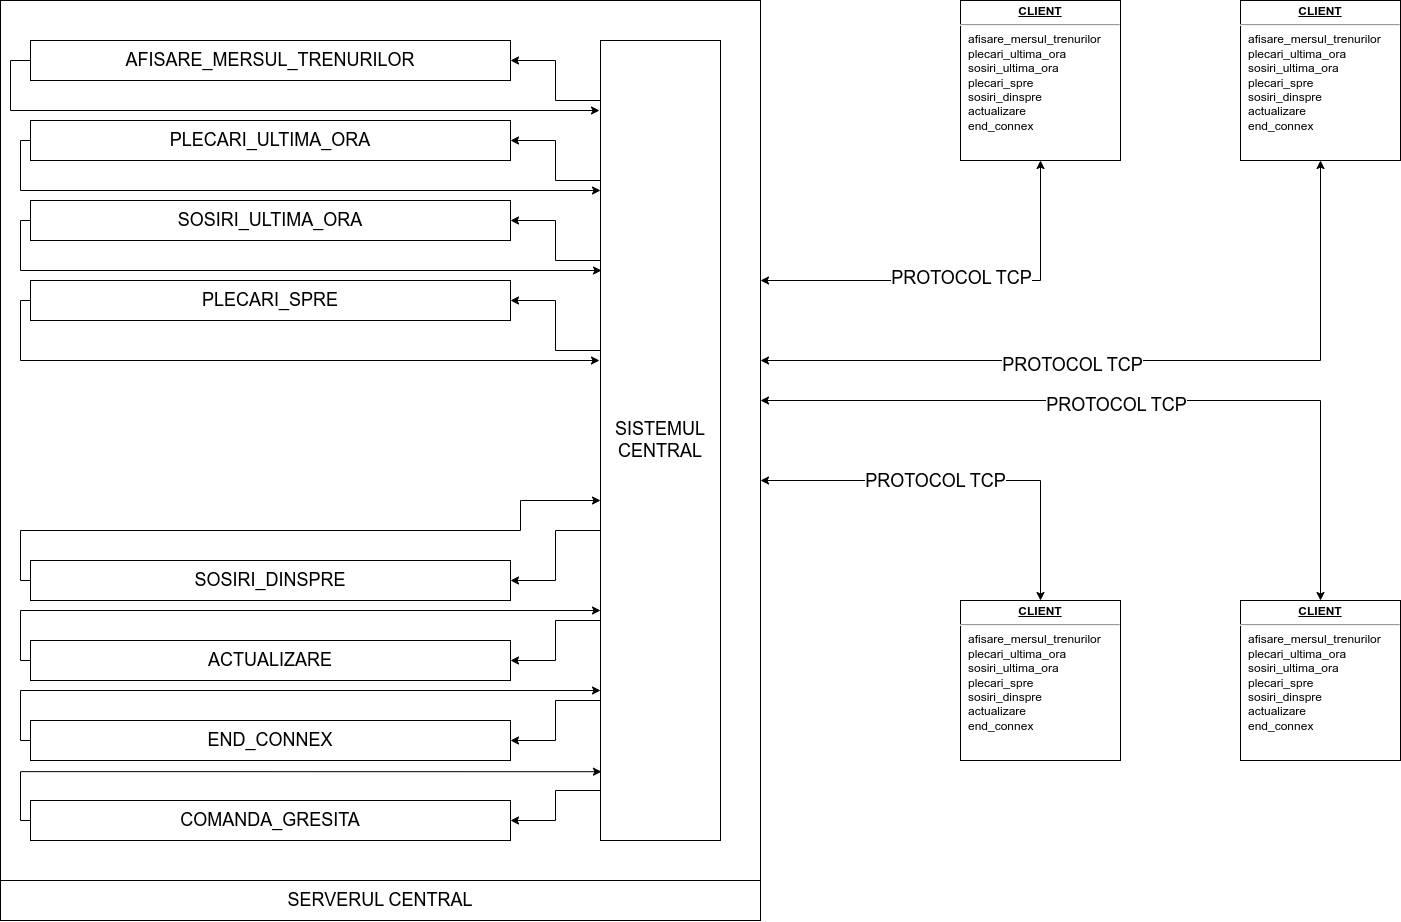
\includegraphics[width=\textwidth]{Arhitectura_aplicatiei.png}
    \caption{Diagrama aplicației}
\end{figure}
Comenzile transmise de către client sunt trimise spre server, prin intermediul socket-urilor. Acestea, ajunse la server, sunt verificate în componenta SISTEMUL CENTRAL, ce stabilește corectitudinea comenzii și rutina de tratare a acelei comenzi. Dacă comanda furnizată de client este corectă, SISTEMUL CENTRAL va apela una din următoarele componente:
\begin{itemize}
    \item \textit{afisare\_mersul\_trenurilor} = parte din server ce va extrage din fișiere XML date privind circulația trenurilor în ziua respectivă (plecare/sosire, nr. tren, ora, direcția, mențiuni). Această componentă este apelată când clientul transmite comanda afisare\_mersul\_trenurilor;
    \item \textit{plecari\_ultima\_ora} = parte din server ce va extrage din fișiere XML date privind plecările ce vor avea loc în următoarea oră. Acesta va trimite către client nr. trenului, ora la care pleacă. direcția și mențiunile. Această componentă este apelată când clientul transmite comanda plecari\_ultima\_ora;
    \item \textit{sosiri\_ultima\_ora} = parte din server ce va extrage din fișiere XML date privind sosirile ce vor avea loc în următoarea oră. Acesta va trimite către client nr. trenului, ora la care sosește. direcția și mențiunile. Această componentă este apelată când clientul transmite comanda sosiri\_ultima\_ora;
    \item \textit{plecari\_spre} = parte din server ce va extrage din fișiere XML date privind plecările ce vor trece prin stația solicitată de server de la client. Acesta va trimite către client nr. trenului, ora la care pleacă. direcția și mențiunile. Această componentă este apelată când clientul transmite comanda plecari\_spre;
    \item \textit{sosiri\_dinspre} = parte din server ce va extrage din fișiere XML date privind trenurile ce sosesc în gară, dar care au trecut prin stația solicitată de server de la client. Acesta va trimite către client nr. trenului, ora la care sosește. direcția și mențiunile. Această componentă este apelată când clientul transmite comanda sosiri\_dinspre;
    \item \textit{actualizare} = parte din server ce se va ocupa cu modificarea datelor privind circulația trenurilor. Această componentă va solicita de la client următoarele date: parola (pentru a se asigura că cel ce solicită modificarea datelor este un operator), nr. trenului, tipul de modificare (întârzieri, mai devreme, conform cu planul) și minutele. Această componentă este apelată când clientul transmite comanda actualizare;
    \item \textit{end\_connex} = parte din server ce se va ocupa cu închiderea conexiunii dintre server și client. Această componentă este apelată când clientul transmite comanda end\_connex;
    \item \textit{comanda\_gresita} = parte din server ce va transmite clientului faptul că acesta a furnizat o comandă scrisă greșit sau o comandă inexistentă.
\end{itemize}

\section{Detalii de implementare}

\subsection{Implementarea clientului}

Clientul va fi responsabil de transmiterea către server a comenzilor și informațiilor necesare, dar și de afișare a cererilor făcute de server și a răspunsurilor date de acesta. Comunicarea se va realiza prin intermediul socket-ului. Astfel, la început se va realiza procedura standard de creare a socket-ului și de conectare a clientului cu serverul prin intermediul funcției connect().

\begin{verbatim}
    while(1)
    {
        ...
    }
\end{verbatim}
Această buclă while va permite utilizatorului să trimită câte comenzi dorește utilizatorul.

\begin{verbatim}
cout<<"Introduceti comanda: ";
cin.getline(stocare_mesaj_client, 60);   
cout<<endl;
lungime_comanda=strlen(stocare_mesaj_client);
int trimite_lungime_mesaj=write(descriptor_socket, 
&lungime_comanda, sizeof(int)); 
if(trimite_lungime_mesaj==-1)
{
    perror("Eroare la transmiterea lungimii mesajului \n");
    return errno;
}
int scriere_1=write(descriptor_socket, stocare_mesaj_client,
strlen(stocare_mesaj_client));
if(scriere_1==-1)
{
    perror("Eroare la transmiterea comenzii \n");
    return errno;
}
\end{verbatim}
Această porțiune de cod este responsabilă cu: citirea de la tastatură a comenzii date de utilizator; transmiterea lungimii (pentru a înștiința serverul despre numărul de caractere ce vor fi citite) și transmiterea efectivă a comenzii către server. În caz de eșec, clientul va afișa mesajul de avertizare specificat.

\begin{verbatim}
while(rezolvare_comanda==RUNNING)
{
    ...
}
\end{verbatim}
Această buclă while are rolul de a determina dacă serverul mai are nevoie de informații necesare pentru o comanda (comanda actualizare). 

\begin{verbatim}
int lungime_mesaj_receptionat;
int citire_lungime=read(descriptor_socket, 
&lungime_mesaj_receptionat, sizeof(int)); 
int citire_raspunsuri=read(descriptor_socket,
mesaj_primit, lungime_mesaj_receptionat);
int decizie;
int finish_command=read(descriptor_socket, &decizie, sizeof(int));
\end{verbatim}
Această porțiune de cod este responsabilă de receptarea lungimii mesajului, receptarea mesajului și receptarea semnalului de finalizare a comenzii dată de server.

\begin{verbatim}
if(decizie==0)
{
    bzero(stocare_mesaj_client, sizeof(stocare_mesaj_client));
    cout<<mesaj_primit;
    cin.getline(stocare_mesaj_client, 60);   
    cout<<endl;
    bzero(mesaj_primit, sizeof(mesaj_primit)); 
    lungime_comanda=strlen(stocare_mesaj_client);
    int trimite_lungime_mesaj_1=write(descriptor_socket, 
    &lungime_comanda, sizeof(int)); 
    if(trimite_lungime_mesaj_1==-1)
    {
        perror("Eroare la transmiterea lungimii 
        mesajului in while 2 \n");
        return errno;
    }
    int scriere_2=write(descriptor_socket,
    stocare_mesaj_client, strlen(stocare_mesaj_client));
    if(scriere_2==-1)
    {
        perror("Eroare la transmiterea comenzii in while 2 \n");
        return errno;
    }
}
\end{verbatim}
Dacă decizia este 0 (serverul solicită informații suplimentare), clientul va afișa mesajul transmis de server (probabil ce informații trebuie să furnizeze utilizatorul). Apoi clientul va recepta informațiile scrise la tastatură de către utilizator, pe care le va transmite către server.

\begin{verbatim}
else
{
    cout<<mesaj_primit;
    if(strcmp(mesaj_primit, "END_CONNEX\n")==0)
    {
        end_connex=1;
    }
    bzero(stocare_mesaj_client, sizeof(stocare_mesaj_client));
    bzero(mesaj_primit, sizeof(mesaj_primit)); 
    rezolvare_comanda=DONE;
}
\end{verbatim}
Altfel, va afișa informațiile cerute de utilizator. Clientul va face o verificare suplimentară, pentru a verifica dacă mesajul transmis de server este END\_CONNEX (semnal pentru închiderea conexiunii). Variabila rezolvare\_comanda va primi valoarea DONE (pentru a ieși din bucla while).

\begin{verbatim}
if(end_connex==1)
{
    break;
}
\end{verbatim}
Dacă end\_connex este 1, atunci se va ieși din buclă (marchează închiderea conexiunii).
\begin{verbatim}
close(descriptor_socket);
\end{verbatim}
Aici închidem socket-ul.

\subsection{Implementarea serverului}

Se va realiza procedura standard de creare a structurii sockaddr\_in și a socket-ului.
\begin{verbatim}
while(1)
{
    int clientela;
    socklen_t lungime = sizeof(per_client);
    if((clientela = accept(socket_principal, 
    (struct sockaddr*) &per_client, &lungime))<0)
    {
        perror ("server | eroare la accept\n");
        continue;
    }
    pthread_create(&MULTIME[i], NULL, &tratare, &clientela);
    cout<<"thread "<<i<<" creat"<<endl;
    i++;
}
\end{verbatim}
În bucla while, se realizează conectarea serverului cu clienții. Totuși pentru a asigura faptul că serverul este concurent, apelăm la noțiunea de thread. Astfel, după realizarea conexiunii, creăm un thread ce se va ocupa de clientul recent conectat. Acesta va apela funcția tratare(), având ca parametru id-ul clientului.

\begin{verbatim}
static void *tratare (void * arg)
{
    pthread_detach(pthread_self());
    Sistemul_Central((int*)arg);
    printf("Inchis thread\n");
    return NULL;
};
\end{verbatim}
Funcția de tratare va realiza următoarele operații: eliberarea resurselor la finalul execuției thread-ului, apelarea funcției Sistemul\_Central(), responsabilă cu rezolvarea solicitărilor primite de la client, închiderea thread-ului.

\begin{verbatim}
void Sistemul_Central(void *arg)
{
    ... //declarări de variabile
    while(comunicare_client_server == 1)
    {
        ...
    }
    cout<<"Inchis conexiune"<<endl;
    close(client);
}
\end{verbatim}
Funcția Sistemul\_Central este responsabilă cu rezolvarea solicitărilor primite de la client. Această funcția va rula cât timp, clientul nu a trimis comanda end\_connex, comandă ce va modifica valoarea variabilei comunicare\_client\_server. Apoi va închide socket-ul.

Protocolul de comunicare între server și client este următorul: serverul citește de la client lungimea mesajului și mesajul efectiv, apoi serverul transmite înapoi clientului lungimea mesajului, mesajul efectiv și un flag ce semnalizează finalizarea comenzii. Acest flag este important pentru a semnala clientului când serverul are nevoie de informații suplimentare de la utilizator.

\begin{verbatim}
if(strcmp(mesaj_primit, "afisare_mersul_trenurilor")==0)
{
    pthread_mutex_lock(&MUTEX); //necesara pentru a evita 
    //data race
    char rezultat_parsare[8196]; //variabila intermediara
    bzero(rezultat_parsare, 8196);//eliberarea acesteia
    mersul_trenurilor(rezultat_parsare); //functia responsabila
    //de rezolvarea cerintei
    ...//transmiterea mesajului catre client
}
\end{verbatim}
Când serverul a primit comanda afisare\_mersul\_trenurilor, va apela funcția mersul\_trenurilor responsabilă cu extragerea de date din fișiere XML.

\begin{verbatim}
void mersul_trenurilor(char* locatie)
{
    char rezultat[8196];
    bzero(rezultat, 8196);
    pugi::xml_document tabela;
    pugi::xml_parse_result actual =
    tabela.load_file("Planificare_tren.xml");
    ... //linii de cod ce țin de aranjarea în char
    for(pugi::xml_node tren = tabela.child("TABELA").
    child("PLECARI").first_child(); 
    tren; tren = tren.next_sibling())
    {
        char numar[10];
        strcpy(numar, tren.child("NUMAR").
        attribute("nr").value());
        strcat(rezultat, numar);
        int lungime = strlen(numar);
        for(int i=0; i<(8-lungime); i++)
        {
            strcat(rezultat, " ");
        }
        char directie[50];
        strcpy(directie, tren.child("DESTINATIE").
        attribute("dest").value());
        lungime = strlen(directie);
        strcat(rezultat, directie);
        for(int i=0; i<(20-lungime); i++)
        {
            strcat(rezultat, " ");
        }
        char ora[10];
        strcpy(ora, tren.child("ORA").attribute("h").value());
        lungime = strlen(ora);
        strcat(rezultat, ora);
        for(int i=0; i<(8-lungime); i++)
        {
            strcat(rezultat, " ");
        }
        char mentiuni[50];
        strcpy(mentiuni, 
        tren.child("MENTIUNI").attribute("ment").value());
        lungime = strlen(mentiuni);
        strcat(rezultat, mentiuni);
        for(int i=0; i<(24-lungime); i++)
        {
            strcat(rezultat, " ");
        }
        strcat(rezultat, "\n");
    }
    ...//linii de cod ce țin de aranjarea 
    //informației in char
    for(pugi::xml_node tren = tabela.child("TABELA").
    child("SOSIRI").first_child(); 
    tren; tren = tren.next_sibling())
    {
        ...//linii de cod ce țin de extragerea de 
        //date din fisiere XML
    }
    strcpy(locatie, rezultat);
}
\end{verbatim}
Folosind funcțiile oferite de librăria \textbf{pugixml}, realizăm un for peste conținutul ramurii PLECARI, și extragem numărul, direcția, ora și mențiunile fiecărui tren. La fel, facem și pentru ramura SOSIRI.

\begin{verbatim}
else if(strcmp(mesaj_primit, "plecari_ultima_ora")==0)
{
    ...//MUTEX, variabile auxiliare
    deplasari_curente(rezultat_parsare, 1);
    ...//transmiterea mesajului
}
else if(strcmp(mesaj_primit, "sosiri_ultima_ora")==0)
{
    ...//MUTEX, variabile auxiliare
    deplasari_curente(rezultat_parsare, 0);
    ...//transmiterea mesajului
}
\end{verbatim}
Comenzile plecari\_ulitma\_ora și sosiri\_ultima\_ora folosesc funcția deplasari\_curente(), ce primește ca parametrii locația unde să stocheze informația extrasă și o variabilă locatie, care indică ramura de pe care trebuie extrasă informația (1 pentru plecari, 0 pentru sosiri).

\begin{verbatim}
void deplasari_curente(char* locatie, int location)
{
    ...// variabile
    time_t ceas;
    struct tm* information;
    char ora_exacta[8];
    //ora la care se realizeaza comanda
    char ora_viitoare[8];
    //ora + 1
    time(&ceas);
    information = localtime(&ceas);
    strftime(ora_exacta, 8, "%H:%M", information);
    information->tm_hour=(information->tm_hour+1)%24;
    strftime(ora_viitoare, 8, "%H:%M", information);
    //bucata aceasta de cod este responsabila
    //de extragerea orei
    pugi::xml_document tabela;
    pugi::xml_parse_result actual = 
    tabela.load_file("Planificare_tren.xml");
    if(location == 1) //plecari        
    {
        ...//cod pentru aranjarea in char
        for(pugi::xml_node tren = 
        tabela.child("TABELA").child("PLECARI").first_child(); 
        tren; tren = tren.next_sibling())
        {
            char ora[3];
            char minut[3];
            char ora_tabela[100];
            strcpy(ora_tabela, tren.child("ORA").attribute("h").value());
            char* haz;
            haz=strtok(ora_tabela, ":");
            strcpy(ora, haz);
            haz=strtok(NULL, ":");
            strcpy(minut, haz);
            int hour = atoi(ora);
            int hmin = atoi(minut);
            char est[5];
            strcpy(est, tren.child("MENTIUNI").
            attribute("min").value());
            int estim = atoi(est);
            time_t ceas_1;
            struct tm* information_1;
            char ora_necesara[8];
            time(&ceas_1);
            information_1 = localtime(&ceas_1);
            information_1->tm_hour = hour;
            information_1->tm_min = hmin + estim;
            if(information_1->tm_min>=60)
            {
                information_1->tm_hour = (information_1->tm_hour+1)%24;
                information_1->tm_min = information_1->tm_min%60;
            }
            if(information_1->tm_min<0)
            {
                information_1->tm_hour = (information_1->tm_hour+23)%24;
                information_1->tm_min = information_1->tm_min+60;
            }
            strftime(ora_necesara, 8, "%H:%M", information_1);
            if(strcmp(ora_necesara, ora_exacta)>=0
            && strcmp(ora_necesara, ora_viitoare)<=0)
            //verificam daca ora din tabel se afla in intervalul
            //respectiv
            {
                ...//cod pentru extragerea si arajarea
                //in char
            }
        }
        strcpy(locatie, rezultat);
    }
    else//sosiri
    {
        ...//cod asemanator cu ramura plecari
    }
}
\end{verbatim}
Folosind funcțiile din librăriile time.h și pugixml, extragem odată ora la care s-a făcut interogarea. Apoi, pentru fiecare tren construim ora exactă la care sosește/pleacă. Apoi verificăm dacă se află în intervalul orar dorit, iar dacă se află, îl inserăm în răspuns.

\begin{verbatim}
else if(strcmp(mesaj_primit, "plecari_spre")==0)
{
    ...//cod pentru solicitarea de la client a statiei
    ...//cod pentru citirea de la client a statiei
    deplasari_via(rezulate, 1, mesaj_primit);
    ...//transmiterea spre client a informatiei
}
else if(strcmp(mesaj_primit, "sosiri_dinspre")==0)
{
    ...//cod pentru solicitarea de la client a statiei
    ...//cod pentru citirea de la client a statiei
    deplasari_via(rezulate, 0, mesaj_primit);
    ...//transmiterea spre client a informatiei
}
\end{verbatim}
Comenzile plecari\_spre și sosiri\_dinspre solicită suplimentar de la client și o stație necesară efectuării înterogării, iar apoi apelează funcția deplasari\_via(), ce oferă informațiile cerute,
\begin{verbatim}
void deplasari_via(char* locatie, int location, char* via)
{
    char rezultat[8196];
    bzero(rezultat, 8196);
    pugi::xml_document tabela;
    pugi::xml_parse_result actual =
    tabela.load_file("Planificare_tren.xml");
    if(location == 1) //plecari
    {
        ...//cod pentru aranjare
        for(pugi::xml_node tren = 
        tabela.child("TABELA").child("PLECARI").first_child(); 
        tren; tren = tren.next_sibling())
        //primul for pentru parcurgerea fiecarei curse 
        //de pe ramura plecari
        {
                for(pugi::xml_node station = 
                tren.child("STATII").child("GARA"); 
                station; station=station.next_sibling())
                //cod necesar pentru parcurgerea statiilor
                {
                    if(strcmp(via, 
                    station.attribute("gara").value())==0)
                    //daca statia data de client exista pe lista
                    //extrag informatiile
                    {
                        ...//cod pentru extragerea
                        //de informatii
                    }
                }
            }
        }
        else//sosiri
        {
            ...//cod asemanator ramurii plecari
        }
}
\end{verbatim}
Funcția de mai sus parcurge ramura indicată de variabila location și verifică dacă în lista de stații a trenului există stația primită de la client. Dacă există, extrage datele despre acel tren.

\begin{verbatim}
else if(strcmp(mesaj_primit, "actualizare")==0)
{
    ...//cod pentru solicitarea parolei
    //si pentru citirea acesteia
    int corect = check_parola(mesaj_primit);
    if(corect==0)
    {
        ...//tratarea acestui caz
    }
    else
    {
        ...//solicitarea de informatii referitoare 
        //la tren
        //si citirea acestora
        int modification = 
        modificare_planificare(nr_tren, tip_modificare, 
        minute);
        //functia ce realizeaza modificarea
        if(modification == -1)//nr tren gresit/neexistent
        {
            ...//tratarea acestui caz
        }
        else if(modification == -2)//parametru gresit 
        //la tip_modificare
        {
            ...//tratarea acestui caz
        }
        else if(modification == -3)//parametru gresit la 
        //minute
        {
            ...//tratarea acestui caz
        }
        else if(modification == -5)//tren deja plecat
        {
            ...//tratarea acestui caz
        }
        else if(modification == -6)//trenul deja a sosit
        {
            ...//tratarea acestui caz
        }
        else//reusit
        {
            ...//tratarea acestui caz
        }
    }
}
\end{verbatim}
Comanda actualizare solicită suplimentar de la client o parola, iar dacă aceasta este corectă, solicită date referitoare la tren și tipul de modificare. După recepționarea acestor informații, se apelează funcția modificare\_planificare(), ce modifică fișierul XML, dacă informațiile oferite sunt corecte, sau returnează un număr negativ, folosit la semnalarea greșelii produse. Apoi se realizează tratarea fiecărui caz.

\begin{verbatim}
int modificare_planificare(char* nr_tren, 
char* tip_modificare, char* minute)
{
    int gasit=0;
    time_t ceas;
    struct tm* information;
    char ora_exacta[8];
    time(&ceas);
    information = localtime(&ceas);
    strftime(ora_exacta, 8, "%H:%M", information);
    pugi::xml_document tabela;
    pugi::xml_parse_result actual 
    = tabela.load_file("Planificare_tren.xml");
    if(strcmp(tip_modificare, "INT")==0)
    //se solicita intarzierea sosirii unui tren
    {
        if(strcmp(minute, "0")>0 || strcmp(minute, "1440")<=0)
        {
            for(pugi::xml_node tren = 
            tabela.child("TABELA").child("PLECARI").first_child(); 
            tren; tren = tren.next_sibling())
            {
                if(strcmp(nr_tren, 
                tren.child("NUMAR").attribute("nr").value())==0)
                {
                    gasit++;
                    char ora[3];
                    char minut[3];
                    char ora_tabela[100];
                    strcpy(ora_tabela, 
                    tren.child("ORA").attribute("h").value());
                    char* haz;
                    haz=strtok(ora_tabela, ":");

                    strcpy(ora, haz);
                    haz=strtok(NULL, ":");
                    
                    strcpy(minut, haz);
                    int hour = atoi(ora);
                    int hmin = atoi(minut);
                    char est[5];
                    strcpy(est, 
                    tren.child("MENTIUNI").attribute("min").value());
                    int estim = atoi(est);
                    time_t ceas_1;
                    struct tm* information_1;
                    char ora_necesara[8];
                    time(&ceas_1);
                    information_1 = localtime(&ceas_1);
                    information_1->tm_hour = hour;
                    information_1->tm_min = hmin + estim;
                    if(information_1->tm_min>=60)
                    {
                        information_1->tm_hour = 
                        (information_1->tm_hour+1)%24;
                        information_1->tm_min = 
                        information_1->tm_min%60;
                    }
                    if(information_1->tm_min<0)
                    {
                        information_1->tm_hour = 
                        (information_1->tm_hour+23)%24;
                        information_1->tm_min = 
                        information_1->tm_min+60;
                    }
                    strftime(ora_necesara, 8, "%H:%M", information_1);
                    if(strcmp(ora_exacta, ora_necesara)<0)
                    {
                        char nou[100];
                        strcpy(nou, "Intarziere: ");
                        strcat(nou, minute);
                        strcat(nou, " minute.");
                        tren.child("MENTIUNI").attribute("ment").
                        set_value(nou);
                        tren.child("MENTIUNI").attribute("min").
                        set_value(minute);
                        tabela.save_file("Planificare_tren.xml");
                        break;
                    }
                    else
                    {
                        return -5; //este plecat
                    }
                }
            }
            for(pugi::xml_node tren = 
            tabela.child("TABELA").child("SOSIRI").first_child(); 
            tren; tren = tren.next_sibling())
            {
                ...//actualizare la sosiri
            }
            if(gasit > 0)
            {
                return 0;
            }
            else
            {
                return -1;
            }
        }
        else
        {
            return -3;
        }
    }
    else if(strcmp(tip_modificare, "DEV")==0)
    //se solicita ajungerea mai devreme a unui tren
    {
        if(strcmp(minute, "0")>0 || strcmp(minute, "1440")<=0)
        {
            for(pugi::xml_node tren 
            = tabela.child("TABELA").child("SOSIRI").first_child(); 
            tren; tren = tren.next_sibling())
            {
                if(strcmp(nr_tren, 
                tren.child("NUMAR").attribute("nr").value())==0)
                {
                    gasit++;
                    char ora[3];
                    char minut[3];
                    char ora_tabela[100];
                    strcpy(ora_tabela, 
                    tren.child("ORA").attribute("h").value());
                    char* haz;
                    haz=strtok(ora_tabela, ":");
                    strcpy(ora, haz);
                    haz=strtok(NULL, ":");
                    strcpy(minut, haz);
                    int hour = atoi(ora);
                    int hmin = atoi(minut);
                    char est[5];
                    strcpy(est, 
                    tren.child("MENTIUNI").attribute("min").value());
                    int estim = atoi(est);
                    time_t ceas_1;
                    struct tm* information_1;
                    char ora_necesara[8];
                    time(&ceas_1);
                    information_1 = localtime(&ceas_1);
                    information_1->tm_hour = hour;
                    information_1->tm_min = hmin + estim;
                    if(information_1->tm_min>=60)
                    {
                        information_1->tm_hour = 
                        (information_1->tm_hour+1)%24;
                        information_1->tm_min = 
                        information_1->tm_min%60;
                    }
                    if(information_1->tm_min<0)
                    {
                        information_1->tm_hour = 
                        (information_1->tm_hour+23)%24;
                        information_1->tm_min = 
                        information_1->tm_min+60;
                    }
                    strftime(ora_necesara, 8, "%H:%M", information_1);
                    if(strcmp(ora_exacta, ora_necesara)<0)
                    {
                        char nou[100];
                        strcpy(nou, "Mai devreme cu ");
                        strcat(nou, minute);
                        strcat(nou, " minute.");
                        char decam[5];
                        strcpy(decam, "-");
                        strcat(decam, minute);
                        tren.child("MENTIUNI").
                        attribute("ment").set_value(nou);
                        tren.child("MENTIUNI").
                        attribute("min").set_value(decam);
                        tabela.save_file("Planificare_tren.xml");
                        break;
                    }
                    else
                    {
                        return -6; //deja sosit
                    }
                }
            }
            for(pugi::xml_node tren 
            = tabela.child("TABELA").child("PLECARI").first_child(); 
            tren; tren = tren.next_sibling())
            {
               ...//actualizare pe ramura plecari
            }
            if(gasit > 0)
            {
                return 0;
            }
            else
            {
                return -1;
            }
        }
        else
        {
            return -3;
        }
    }
    else if(strcmp(tip_modificare, "CCP")==0)
    //se solicita respectarea planului
    {
        for(pugi::xml_node tren = 
        tabela.child("TABELA").child("PLECARI").first_child(); 
        tren; tren = tren.next_sibling())
        {
            ...//actualizare pe ramura plecari
        }
        for(pugi::xml_node tren = 
        tabela.child("TABELA").child("SOSIRI").first_child(); 
        tren; tren = tren.next_sibling())
        {
            ...//actualizare ramura sosiri
        }
        if(gasit > 0)
        {
            return 0;
        }
        else
        {
            return -1;
        }
    }
    else
    {
        return -2;
    }
}
\end{verbatim}
Funcția modificare\_planificare() extrage prima oară ora la care s-a trimis comanda. Apoi se verifică corectitudinea parametrului legat de tipul de modificare. Apoi se verifică corectitudinea timpului (acesta nu trebuie să depășească 24 de ore). După aceea, se va parcurge lista cu trenuri și, în caz de există trenul cu numărul respectiv, sa extragă ora la care acesta sosește/pleacă și să verifice dacă nu cumva acesta a sosit deja în stație, respectiv a plecat din stație. Apoi se va efectua modificările de rigoare.  În caz contrar, acesta returnează un număr negativ, ce va fi tratat de Sistemul\_Central.

\begin{verbatim}
else if(strcmp(mesaj_primit, "end_connex")==0)
{
    ...//tratare
}
\end{verbatim}
În secțiunea dedicată comenzii end\_connex, serverul va trimite un mesaj clientului, apoi va asigna variabilei comunicare\_client\_server valoarea 0, ca acesta să oprească bucla while. 
\begin{verbatim}
else//comanda gresita
{
    ...//tratare
}
\end{verbatim}
Dacă comanda transmisă de client nu se regăsește în lista de comenzi știute de server, acesta va trimite clientului mesajul „Comanda furnizata nu este corecta!”.

\begin{verbatim}
close(client);
\end{verbatim}
Aici se realizează închiderea conexiunii.

\subsection{Scenarii de utilizare}

 \subsubsection{Scenariul 1.} 
 Utilizatorul dorește să afle ce trenuri circulă în ziua respectivă. Astfel trimite comanda \textit{afisare\_mersul\_trenurilor} aplicației client. Clientul trimite comanda primită serverului. Serverul, prin intermediul funcției Sistemul\_Central(), intră pe ramura afisare\_mersul\_trenurilor. Ramura respectivă va genera un char* ce conține date extrase din fișierul XML privitoare la circulația trenurilor din ziua respectivă. Clientul, după ce primește răspunsul, va afișa în consolă datele.
 \begin{figure}[H]
    \centering
    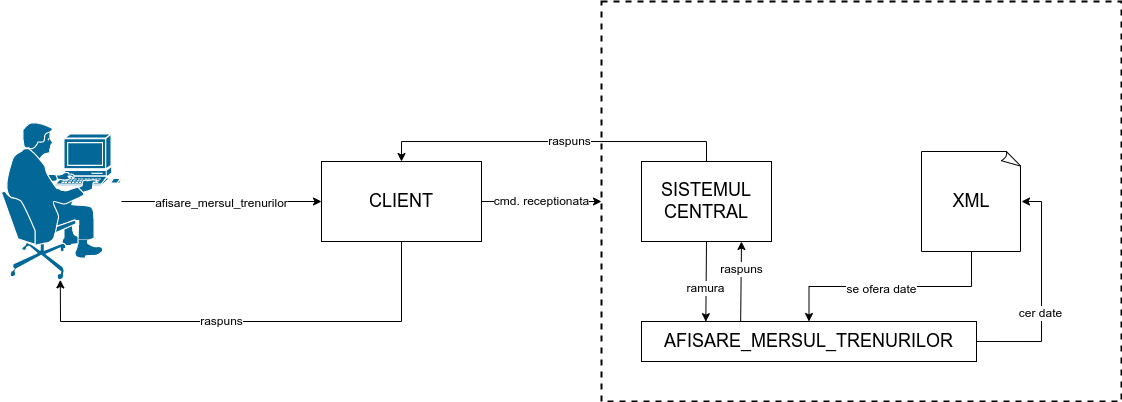
\includegraphics[width=\textwidth]{scenariu_afisare.png}
\end{figure}

 \subsubsection{Scenariul 2.} 
 Utilizatorul dorește să afle ce trenuri pleacă în următoarea oră. Acesta trimite comanda \textit{plecari\_ultima\_ora} aplicației client. Clientul trimite comanda primită serverului. Serverul, prin intermediul funcției Sistemul\_Central(), intră pe ramura plecari\_ultima\_ora.  Această ramură va determina ora la care s-a efectuat cererea, apoi va căuta în fișierul XML plecările din următoarea oră. Datele extrase sunt stocate într-un char* ce va fi livrat aplicației client. Clientul, după ce primește răspunsul, va afișa în consolă datele.

\begin{figure} [H]
    \centering
    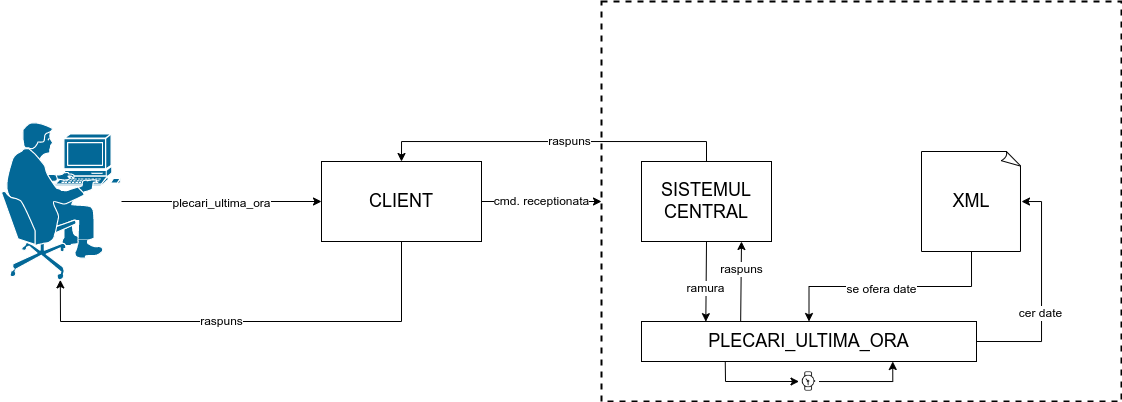
\includegraphics[width=\textwidth]{scenariu_plecari_ora.png}
\end{figure}
 \subsubsection{Scenariul 3.}
  Utilizatorul dorește să afle ce trenuri sosesc în următoarea oră. Acesta trimite comanda \textit{sosiri\_ultima\_ora} aplicației client. Clientul trimite comanda primită serverului. Serverul, prin intermediul funcției Sistemul\_Central(), intră pe ramura sosiri\_ultima\_ora.  Această ramură va determina ora la care s-a efectuat cererea, apoi va căuta în fișierul XML sosirile din următoarea oră. Datele extrase sunt stocate într-un char* ce va fi livrat aplicației client. Clientul, după ce primește răspunsul, va afișa în consolă datele.

\begin{figure} [H]
    \centering
    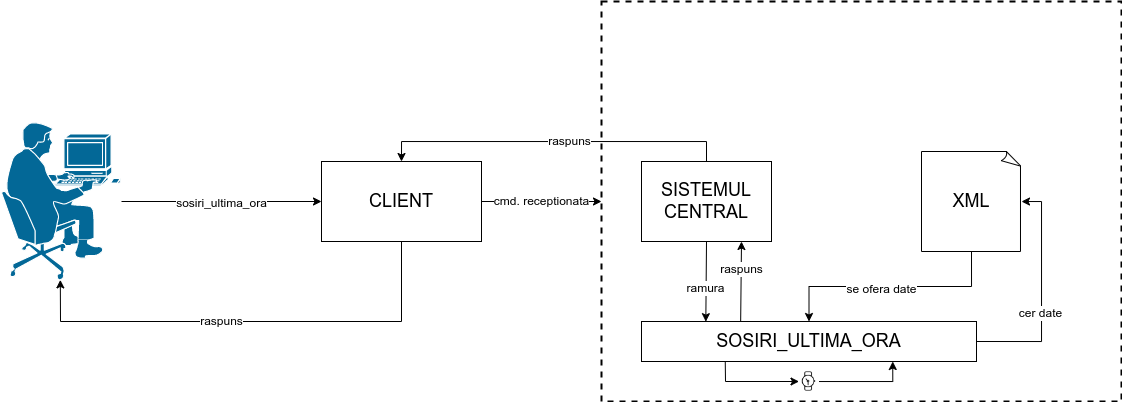
\includegraphics[width=\textwidth]{scenariu_sosiri_ora.png}
\end{figure}

 \subsubsection{Scenariul 4.}
   Utilizatorul dorește să afle trenurile ce vor trece printr-o anumită stație.  Acesta trimite comanda \textit{plecari\_spre} aplicației client. Clientul trimite comanda primită serverului. Serverul, prin intermediul funcției Sistemul\_Central(), intră pe ramura plecari\_spre.  Această ramură va solicita utilizatorului stația, apoi va căuta în fișierul XML plecările ce vor trece prin acea stație. Datele extrase sunt stocate într-un char* ce va fi livrat aplicației client. Clientul, după ce primește răspunsul, va afișa în consolă datele.

\begin{figure} [H]
    \centering
    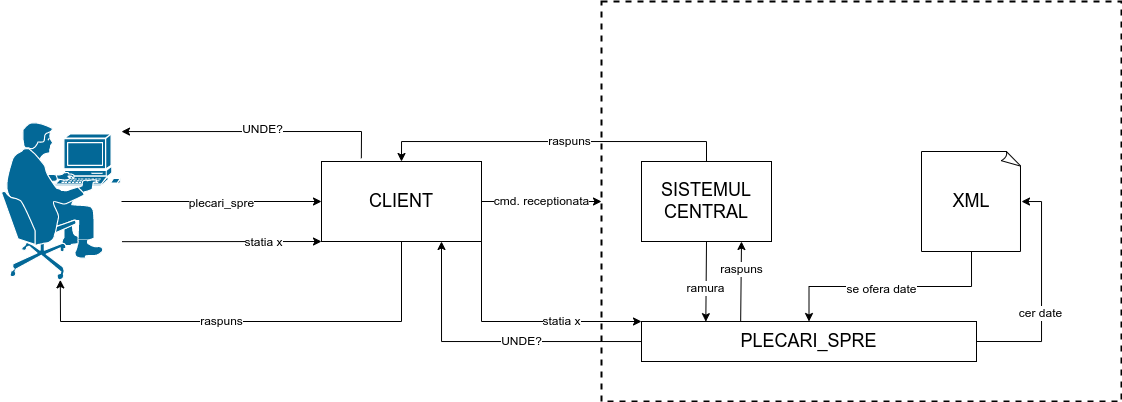
\includegraphics[width=\textwidth]{scenariu_plecari_spre.png}
\end{figure}

 \subsubsection{Scenariul 5.}
    Utilizatorul dorește să afle trenurile ce vin dintr-o anumită stație. Acesta trimite comanda \textit{sosiri\_dinspre} aplicației client. Clientul trimite comanda primită serverului. Serverul, prin intermediul funcției Sistemul\_Central(), intră pe ramura sosiri\_dinspre.  Această ramură va solicita utilizatorului stația, apoi va căuta în fișierul XML sosirile ce au trecut prin acea stație. Datele extrase sunt stocate într-un char* ce va fi livrat aplicației client. Clientul, după ce primește răspunsul, va afișa în consolă datele.

\begin{figure} [H]
    \centering
    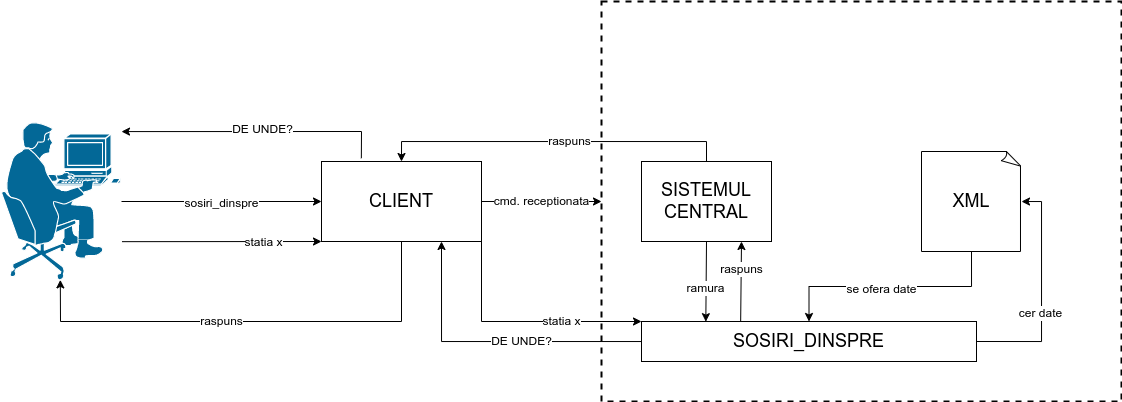
\includegraphics[width=\textwidth]{scenariu_sosiri_dinspre.png}
\end{figure}

 \subsubsection{Scenariul 6.}
 Utilizatorul dorește să actualizeze date privind circulația trenurilor. Acesta trimite comanda \textit{actualizare} aplicației client. Clientul trimite comanda primită serverului. Serverul, prin intermediul funcției Sistemul\_Central(), intră pe ramura actualizare. Serverul va solicita parola, deoarece serverul dorește să determine dacă cel ce va modifica datele este operatorul sau călătorul. 

Dacă parola furnizată de utilizator este corectă, atunci serverul va solicita utilizatorului nr. trenului, dacă modificarea este întârziere/mai devreme/conform cu planul, și minutele. Dacă parametrii sunt corecți, va efectua modificarea, returnând utilizatorului mesajul \textit{Modificare reusita}. Altfel returnează din ce cauză nu s-a efectuat modificarea. Dacă parola este incorectă, atunci serverul va trimite mesajul \textit{PAROLA INCORECTA! ACCES INTERZIS}. 
 \begin{figure}[H]
     \centering
     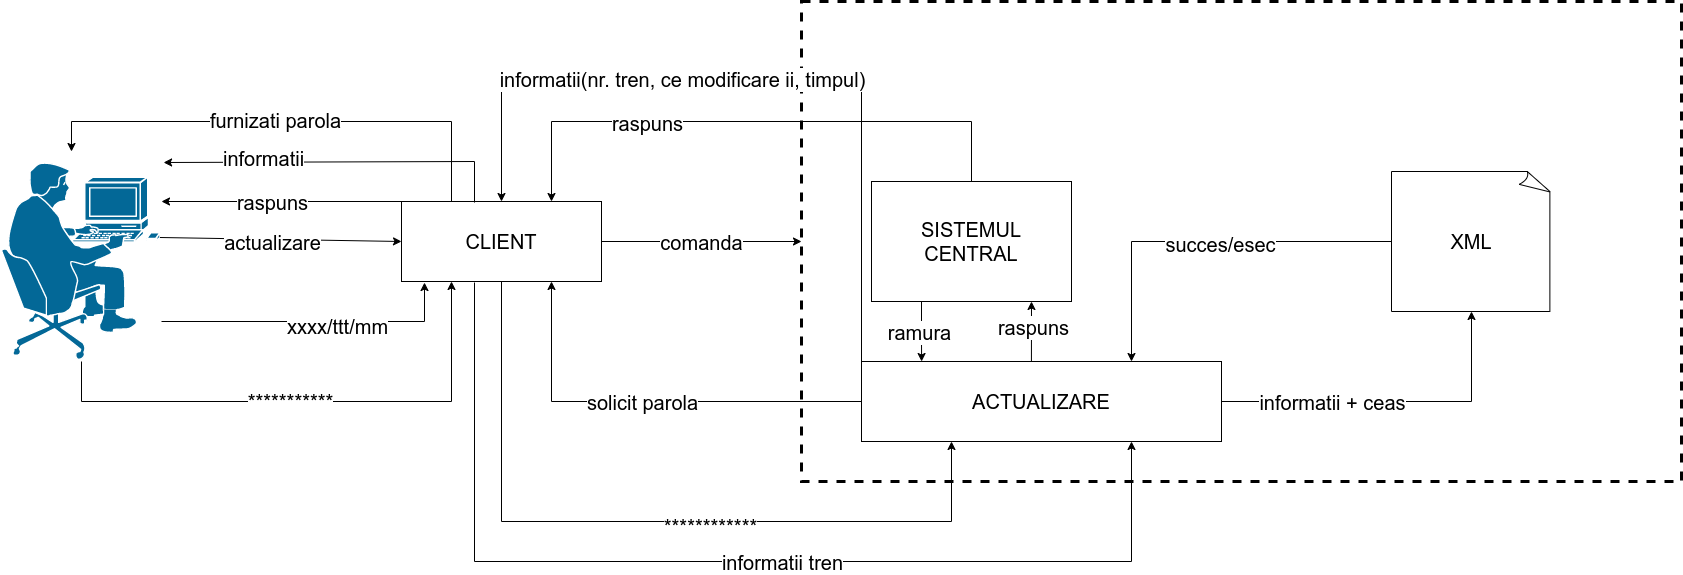
\includegraphics[width=\textwidth]{diagrama_use_case_actualizare.png}
 \end{figure}
 \subsubsection{Scenariul 7.}
 Utilizatorul dorește să închidă conexiunea. Acesta trimite comanda \textit{end\_connex} aplicației client. Clientul trimite comanda recepționată serverului. Serverul, prin intermediul funcției Sistemul\_Central(), va intra pe ramura end\_connex. Aceasta transmite înainte mesajul END\_CONNEX, iar apoi se va închide conexiunea. Clientul la recepția acestui mesaj va închide și el conexiunea.
 
 \subsubsection{Scenariul 8.}
 Utilizatorul trimite o comandă greșită sau neexistentă. Acesta trimite acea comandă aplicației client. Clientul trimite comanda primită serverului. Serverul, prin intermediul funcției Sistemul\_Central(), va determina că nu există acea comandă și intră pe ramura de tratare a acestei erori. Serverul transmite mesajul \textit{Comanda furnizata nu este corecta!}, ce va fi transmisă și utilizatorului. 

\section{Concluzii}

Aplicația \textit{Mersul trenurilor} reprezintă o aplicație tip server-client, construită pe baza protocolului TCP, ce oferă informații utilizatorului referitoare la circulația trenurilor, dar care permite administratorilor modificarea acestor date pentru informarea corectă a tuturor utilizatorilor acestei aplicații.  

Sperăm în viitor să oferim aplicației client o interfață grafică intuitivă, astfel încât, utilizatorul să aibă o experiență cât mai plăcută, dar și o funcție de \textit{help} ar fi  benefică.

\begin{thebibliography}{8}
\bibitem{ref_url1}
TechTarget, Transmission Control Protocol (TCP), \url{https://www.techtarget.com/searchnetworking/definition/TCP}. Ultima accesare: 1 Decembrie 2022

\bibitem{ref_url2}
IBM, Transmission Control Protocol, \url{https://www.ibm.com/docs/ro/aix/7.1?topic=protocols-transmission-control-protocol}. Ultima accesare: 2 Decembrie 2022

\bibitem{ref_url3}
RFC 768: User Datagram Protocol, \url{https://www.rfc-editor.org/rfc/rfc768}.
Ultima accesare: 2 Decembrie 2022

\bibitem{ref_url4}
Laboratorul 12, \url{https://profs.info.uaic.ro/~georgiana.calancea/Laboratorul_12.pdf}. Ultima accesare: 2 Decembrie 2022

\bibitem{ref_url5}
Introduction. pugixml 1.13 quick start guide, \url{https://pugixml.org/docs/quickstart.html#introduction}.  Ultima accesare: 2 Decembrie 2022

\end{thebibliography}
\end{document}
